\documentclass[11pt]{article}
\usepackage[margin=1in]{geometry}
\usepackage{amsmath,amssymb,amsthm,mathtools}
\usepackage{graphicx,booktabs,hyperref}
\usepackage[capitalise]{cleveref}

\newtheorem{theorem}{Theorem}
\newtheorem{proposition}[theorem]{Proposition}
\newtheorem{corollary}[theorem]{Corollary}
\newtheorem{lemma}[theorem]{Lemma}
\theoremstyle{remark}
\newtheorem{remark}[theorem]{Remark}
\theoremstyle{definition}
\newtheorem{observation}[theorem]{Numerical observation}

\newcommand{\ip}[2]{\langle #1,#2\rangle}
\newcommand{\R}{\mathbb{R}}

\title{Friction keeps the conservation laws of training alive:\\ exact drift identities for heavy ball and Nesterov momentum}
\author{Pragyaan Gaur}
\date{October 2026}

\begin{document}
\maketitle

\begin{abstract}
Gradient flow on a network with a linear symmetry conserves a quadratic quantity, such as the balancedness $\|w\|^2-a^2$ of a ReLU neuron, the matrix $W_1W_1^\top-W_2^\top W_2$ of a linear network or the norm of scale-invariant weights. Momentum is known to destroy these laws, and the differential equation for how they move is known from work on Noether's theorem in learning dynamics. We turn that equation into quantitative statements. For heavy ball, $m\ddot\theta+\gamma\dot\theta=-\nabla L$, the drift is bounded uniformly in time by $2m\|A\|(L_0-L_\infty)/\gamma^2$, the constant is attained for scale-invariant parameters, and we prove the first-order formula $\lim_{m\to0}(Q_\infty-Q_0)/m=(2/\gamma^3)\int\ip{\nabla L}{A\nabla L}$ along gradient flow. In discrete time we give exact identities with explicit weights for heavy ball and for Nesterov's method with the gradient at the extrapolated point, a bound of order $\eta/(1-\beta)^2$ for constant momentum, and a nuclear-norm bound for linear networks. With Nesterov's schedule $\beta_k=(k-1)/(k+2)$ the weights grow linearly, and for positive semidefinite generators, including scale-invariant weights, we prove that the drift stays above a positive constant independent of the step size, while for heavy ball it vanishes linearly in the step. For indefinite generators this dichotomy is observed numerically. On diagonal linear networks the drift moves the learned solution away from the gradient flow solution and makes it less sparse. The identities and finite-time bounds are formalised in Lean~4 with Mathlib, and the first-order formula and the passages to infinite time are proved on paper.
\end{abstract}

\section{Introduction}

Plain gradient descent is the overdamped limit of a ball rolling on the loss surface through a viscous fluid. Momentum puts the mass back. Polyak's heavy ball method is the discretisation of $m\ddot\theta+\gamma\dot\theta=-\nabla L(\theta)$, and Nesterov's method has the continuum limit $\ddot\theta+(3/t)\dot\theta=-\nabla L(\theta)$ in which the friction fades with time~\cite{polyak1964,su2016}. This paper asks what the friction does to the symmetries of a network.

When the loss is invariant under a one-parameter group $\theta\mapsto e^{sA}\theta$, the gradient is orthogonal to the generator, $\ip{\nabla L(\theta)}{A\theta}=0$. For symmetric $A$ this makes $Q_A(\theta)=\ip{\theta}{A\theta}$ a conserved quantity of gradient flow. The rescaling symmetry of a ReLU neuron gives the balancedness $\|w\|^2-a^2$ and the $GL(r)$ symmetry of a two-layer linear network gives $W_1W_1^\top-W_2^\top W_2$~\cite{du2018,arora2018}.

\paragraph{What is known.} Kunin et al.~\cite{kunin2021} derived, for the scale and rescale symmetries, the second-order equation that these quantities obey under momentum, a damped oscillator driven by the kinetic term, and solved it with a Green's function. Tanaka and Kunin~\cite{tanaka2021} wrote the general version for any symmetry and any Bregman Lagrangian, which includes the time-dependent friction of Nesterov's method: the Noether charge $P=\ip{\dot\theta}{A\theta}$ obeys $\dot P=K-(\text{damping})P$ with $K=\ip{\dot\theta}{A\dot\theta}$. Marcotte, Gribonval and Peyr\'e characterised the complete set of conservation laws of gradient flows~\cite{marcotte2023}. They then showed that under momentum the laws become time dependent, found them for linear networks, and proved that for ReLU networks none survive~\cite{marcotte2024}. For skew-symmetric $A$ one has $K=0$ and $Q\equiv0$, and the equation above reduces to their laws $e^{\gamma t/m}P=\text{const}$. For plain gradient descent, Du, Hu and Lee bounded the drift of balancedness by the sum of squared steps~\cite{du2018}, and Medeiros studied how it scales with the step size near the edge of stability~\cite{medeiros2026}. For diagonal linear networks, Papazov, Pesme and Flammarion showed that momentum enters through $\lambda=\eta/(1-\beta)^2$ and acts through the asymptotic balancedness~\cite{papazov2024}, and Lyu et al.\ characterised the implicit bias of heavy ball and of Nesterov's method with fixed momentum~\cite{lyu2025}. Josz and Li proved that heavy ball preserves boundedness of trajectories as the mass vanishes~\cite{josz2024}. For scale-invariant weights it is known that momentum makes the norm grow~\cite{arora2019,wan2021}.

\paragraph{What is new.} None of these works bounds the drift under momentum. The non-existence result of Marcotte et al.\ leaves open how badly the laws fail, and the differential equation alone does not say. Our results are the following.

\begin{enumerate}
\item A uniform-in-time bound on the drift under heavy ball, proportional to $m/\gamma^2$ times the energy dissipated, with the sharp constant attained by scale-invariant parameters (\cref{thm:hb}, Proposition~\ref{prop:sharp}).
\item A proof of the first-order formula in the mass, using the boundedness theorem of Josz and Li to verify its main hypothesis (\cref{thm:first}).
\item Exact discrete identities with explicit weights for heavy ball with any schedule, a bound of order $\eta/(1-\beta)^2$ for constant momentum, and a nuclear-norm bound for linear networks (\cref{thm:disc,thm:discbound}, Corollary~\ref{cor:matrix}). This extends the $\lambda$ of Papazov et al.\ to every network with a linear symmetry.
\item An exact identity for Nesterov's method with the gradient at the extrapolated point (\cref{thm:nag}), and a proof that with Nesterov's schedule the drift of a positive semidefinite law stays above a step-independent constant while heavy ball's vanishes (\cref{thm:nestlower}, Corollary~\ref{cor:dichotomy}). For indefinite generators we observe the same dichotomy numerically (Observation~\ref{obs:dichotomy}).
\item A demonstration on diagonal linear networks that the drift is the mechanism by which momentum changes the implicit bias (\cref{sec:bias}).
\item A Lean~4 formalisation of the identities and finite-time bounds above. The first-order formula, the passages to infinite time and two short final steps are proved on paper (\cref{sec:lean}).
\end{enumerate}

\section{Setting}\label{sec:setting}

Parameters live in a real inner product space $E$. A bounded linear map $A:E\to E$ is symmetric, $\ip{Ax}{y}=\ip{x}{Ay}$, and generates a symmetry of the loss in the sense that
\begin{equation}\label{eq:orth}
\ip{\nabla L(\theta)}{A\theta}=0\qquad\text{for all }\theta .
\end{equation}
We write $Q(\theta)=\ip{\theta}{A\theta}$, and along a trajectory with velocity $v$ we write $P=\ip{v}{A\theta}$ and $K=\ip{v}{Av}$. Under gradient flow $\dot Q=2P=-2\ip{\nabla L}{A\theta}/\gamma=0$. The only facts about the network that we use are \eqref{eq:orth} and the bound $|K|\le\|A\|\,\|v\|^2$.

Three examples cover the main cases, and the first two include the laws that Marcotte et al.\ found for two-layer linear and ReLU networks. For a ReLU neuron $x\mapsto a\,\sigma(w\cdot x)$, $A$ is $-1$ on $a$ and $+1$ on $w$, so $Q=\|w\|^2-a^2$ and $\|A\|=1$. For a two-layer linear network and a symmetric matrix $X$, the generator $A_X(W_1,W_2)=(XW_1,-W_2X)$ gives $Q=\operatorname{tr}(XC)$ with $C=W_1W_1^\top-W_2^\top W_2$, and $\|A_X\|=\|X\|_{\mathrm{op}}$. For a block $w$ on which the loss is scale invariant, as happens before a normalisation layer, $A$ is the identity on $w$, $Q=\|w\|^2$ and $K=\|\dot w\|^2\ge0$.

\section{Heavy ball in continuous time}\label{sec:hb}

\begin{theorem}\label{thm:hb}
Let $m\ge0$, $\gamma>0$ and let $\theta$ solve $m\ddot\theta+\gamma\dot\theta=-\nabla L(\theta)$ with $\nabla L$ satisfying \eqref{eq:orth}. Then the corrected quantity $\gamma Q+2mP$ satisfies
\begin{equation}\label{eq:hbid}
\frac{d}{dt}\bigl(\gamma Q+2mP\bigr)=2mK ,
\end{equation}
and with $E=\tfrac m2\|\dot\theta\|^2+L(\theta)$, for every $T\ge0$,
\begin{equation}\label{eq:hbbound}
\bigl|\gamma\,(Q(T)-Q(0))+2m\,(P(T)-P(0))\bigr|\le\frac{2m\|A\|}{\gamma}\,\bigl(E(0)-E(T)\bigr).
\end{equation}
If the motion starts at rest and $\dot\theta(T)\to0$ with $\theta$ bounded, then
\begin{equation}\label{eq:hblim}
Q(\infty)-Q(0)=\frac{2m}{\gamma}\int_0^\infty K\,dt,\qquad |Q(\infty)-Q(0)|\le\frac{2m\|A\|}{\gamma^2}\bigl(L(\theta_0)-L_\infty\bigr).
\end{equation}
\end{theorem}

\begin{proof}
Differentiating gives $\dot Q=2P$ by symmetry of $A$, and $\dot P=K+\ip{\ddot\theta}{A\theta}$. Pairing the equation of motion with $A\theta$ and using \eqref{eq:orth} gives $m\ip{\ddot\theta}{A\theta}+\gamma P=0$. Hence $\frac{d}{dt}(\gamma Q+2mP)=2\gamma P+2mK+2m\ip{\ddot\theta}{A\theta}=2mK$. The energy satisfies $\dot E=\ip{m\ddot\theta+\nabla L}{\dot\theta}=-\gamma\|\dot\theta\|^2$, so $\gamma\int_0^T\|\dot\theta\|^2=E(0)-E(T)$. Integrating \eqref{eq:hbid} and using $|K|\le\|A\|\|\dot\theta\|^2$ gives \eqref{eq:hbbound}. Under the extra assumptions $P(0)=0$, $P(T)\to0$ and $E(T)\to L_\infty$, which gives \eqref{eq:hblim}.
\end{proof}

The differential identity \eqref{eq:hbid} is the integrated form of the Noether learning dynamics of Tanaka and Kunin~\cite{tanaka2021} specialised to heavy ball, and for the scale and rescale symmetries it is equivalent to the equations of Kunin et al.~\cite{kunin2021}. The new content of \cref{thm:hb} is the uniform bound \eqref{eq:hbbound} obtained by pairing it with energy dissipation. In the overdamped limit $m\to0$ the law becomes exact again, and the bound says that what breaks it is the dimensionless ratio of inertia to friction times the energy that the friction has to absorb.

\begin{proposition}[sharpness]\label{prop:sharp}
The constant in \eqref{eq:hblim} cannot be improved. For a scale-invariant block with all other parameters fixed, $K=\|\dot\theta\|^2$ and the second statement in \eqref{eq:hblim} holds with equality.
\end{proposition}

\begin{proof}
With $A$ the identity, $K=\|\dot\theta\|^2$, so $\int_0^\infty K=\int_0^\infty\|\dot\theta\|^2=(E(0)-E(\infty))/\gamma$ and the first identity in \eqref{eq:hblim} becomes $\|w_\infty\|^2-\|w_0\|^2=2m(L(\theta_0)-L_\infty)/\gamma^2$.
\end{proof}

The rescaling symmetry of a ReLU neuron also approaches the constant. For $L(a,w)=\tfrac12(aw-1)^2$ started at rest from $(R,0)$ with $m=0.05$ and $\gamma=1$, the ratio of the drift to the bound is $0.832$, $0.985$, $0.9992$, $0.9997$ and $0.99993$ for $R=1,2,4,8,16$. In this unbalanced regime almost all the motion is in $w$, so $K$ is close to $\|\dot\theta\|^2$. For typical initialisations the bound is loose. On the two-layer linear network of \cref{sec:numerics} the ratio is about $0.02$, because the kinetic energy is spread over many parameters and $K$ only sees the part along the generator, with both signs.

\begin{theorem}[first order in the mass]\label{thm:first}
Fix $\gamma>0$ and $\theta_0$, and let $\theta_m$ solve $m\ddot\theta+\gamma\dot\theta=-\nabla L(\theta)$ from rest at $\theta_0$, and $\varphi$ solve $\gamma\dot\varphi=-\nabla L(\varphi)$ from $\theta_0$. Assume that
\begin{enumerate}
\item[(H1)] there is a compact convex set $B$ containing $\varphi([0,\infty))$ and $\theta_m([0,\infty))$ for all $m\in(0,m_0]$, on which $\|\nabla L\|\le G$ and $\nabla L$ is $H$-Lipschitz;
\item[(H2)] the gradient flow reaches the infimum of the loss, $L(\varphi(t))\to L_*:=\inf L$.
\end{enumerate}
Then for each $m\le m_0$ the limit $Q_m(\infty)=\lim_{t\to\infty}Q(\theta_m(t))$ exists, and
\[
\lim_{m\to0}\frac{Q_m(\infty)-Q(\theta_0)}{m}=\frac{2}{\gamma^3}\int_0^\infty\ip{\nabla L(\varphi)}{A\nabla L(\varphi)}\,dt .
\]
\end{theorem}

Hypothesis (H2) holds whenever training interpolates, as in all our examples. For (H1), Josz and Li~\cite{josz2024} proved that if $L$ is $C^{1,1}_{\mathrm{loc}}$, bounded below and definable in an o-minimal structure, which covers networks with ReLU and polynomial activations and squared loss, then heavy ball trajectories are bounded uniformly in small $m$ if and only if gradient flow trajectories are bounded. Under their assumptions (H1) therefore reduces to boundedness of gradient flow.

\begin{lemma}\label{lem:layer}
Under (H1), for all $t\ge0$ and $m\le m_0$,
\[
\|\dot\theta_m(t)\|\le\frac G\gamma,\qquad
\Bigl\|\dot\theta_m(t)+\frac{\nabla L(\theta_m(t))}{\gamma}\Bigr\|\le\frac{HGm}{\gamma^3}+\frac G\gamma e^{-\gamma t/m}.
\]
\end{lemma}

\begin{proof}
Variation of constants with $\dot\theta_m(0)=0$ gives $\dot\theta_m(t)=-\frac1m\int_0^te^{-\gamma(t-u)/m}\nabla L(\theta_m(u))\,du$, so $\|\dot\theta_m\|\le G/\gamma$. Adding $\nabla L(\theta_m(t))/\gamma$ and using $\frac1m\int_0^te^{-\gamma(t-u)/m}du=\frac1\gamma(1-e^{-\gamma t/m})$,
\[
\dot\theta_m(t)+\frac{\nabla L(\theta_m(t))}{\gamma}=-\frac1m\int_0^te^{-\gamma(t-u)/m}\bigl(\nabla L(\theta_m(u))-\nabla L(\theta_m(t))\bigr)du+\frac{e^{-\gamma t/m}}{\gamma}\nabla L(\theta_m(t)).
\]
The difference of gradients is at most $H\|\theta_m(u)-\theta_m(t)\|\le HG(t-u)/\gamma$, and $\frac1m\int_0^\infty e^{-\gamma x/m}x\,dx=m/\gamma^2$.
\end{proof}

\begin{proof}[Proof of \cref{thm:first}]
\emph{Existence of the limit.} The identity of \cref{thm:hb} gives $Q(\theta_m(T))-Q(\theta_0)=\frac{2m}\gamma\int_0^TK\,dt-\frac{2m}\gamma P(T)$. Energy dissipation gives $\int_0^\infty\|\dot\theta_m\|^2\le(L(\theta_0)-L_*)/\gamma$, so the integral converges absolutely. For fixed $m$ the acceleration is bounded on $B$, so $\|\dot\theta_m\|^2$ is uniformly continuous and integrable and tends to zero, and $P(T)\to0$ because $\theta_m$ is bounded.

\emph{Finite horizon.} Let $e=\theta_m-\varphi$. Then $\dot e=\bigl(\dot\theta_m+\nabla L(\theta_m)/\gamma\bigr)+\bigl(\nabla L(\varphi)-\nabla L(\theta_m)\bigr)/\gamma$, so by Lemma~\ref{lem:layer} $\|\dot e\|\le\rho_m(t)+\frac H\gamma\|e\|$ with $\rho_m(t)=HGm/\gamma^3+(G/\gamma)e^{-\gamma t/m}$. Since $\int_0^T\rho_m\le HGmT/\gamma^3+Gm/\gamma^2$, Gr\"onwall gives $\sup_{[0,T]}\|e\|\le C_Tm$. Hence $\|\dot\theta_m-\dot\varphi\|\le\rho_m+\frac H\gamma\|e\|$ and $\int_0^T\|\dot\theta_m-\dot\varphi\|^2\le C'_Tm$, because $\int_0^\infty e^{-2\gamma t/m}dt=m/(2\gamma)$. With both velocities bounded by $G/\gamma$ and Cauchy--Schwarz,
\[
\Bigl|\int_0^TK_m\,dt-\int_0^T\ip{\dot\varphi}{A\dot\varphi}dt\Bigr|\le\|A\|\frac{2G}\gamma\sqrt{T\,C'_Tm}\to0 .
\]

\emph{Tail.} By energy dissipation and $E_m(\infty)\ge L_*$, $\bigl|\int_T^\infty K_m\bigr|\le\|A\|(E_m(T)-L_*)/\gamma$. As $m\to0$, $E_m(T)=\frac m2\|\dot\theta_m(T)\|^2+L(\theta_m(T))\to L(\varphi(T))$ because $\|\dot\theta_m\|\le G/\gamma$ and $\theta_m(T)\to\varphi(T)$. So $\limsup_{m\to0}|\int_T^\infty K_m|\le\|A\|(L(\varphi(T))-L_*)/\gamma$, which tends to $0$ as $T\to\infty$ by (H2). The same bound holds for the gradient flow tail.

Combining the three parts, $\int_0^\infty K_m\to\int_0^\infty\ip{\dot\varphi}{A\dot\varphi}=\gamma^{-2}\int_0^\infty\ip{\nabla L(\varphi)}{A\nabla L(\varphi)}$, and the first identity of \eqref{eq:hblim} finishes the proof.
\end{proof}

Numerically the ratio $(Q_m(\infty)-Q(\theta_0))/m$ on the linear network of \cref{sec:numerics} is $0.3180$ at $m=0.003$ against the limit $0.3146$, and the gap shrinks linearly in $m$. The theorem gives the limit with no rate. The linear rate seen numerically would need more regularity than (H1).

\section{Heavy ball in discrete time}\label{sec:disc}

The iteration is $v_0=-\eta g_0$, $v_{k}=\beta_kv_{k-1}-\eta g_k$, $\theta_{k+1}=\theta_k+v_k$, where $g_k=\nabla L(\theta_k)$ and $\ip{g_k}{A\theta_k}=0$. Write $P_k=\ip{v_k}{A\theta_k}$ and $K_k=\ip{v_k}{Av_k}$.

\begin{theorem}\label{thm:disc}
For any momentum schedule,
\[
Q(\theta_{k+1})-Q(\theta_k)=2P_k+K_k,\qquad P_0=0,\qquad P_{k+1}=\beta_{k+1}(P_k+K_k).
\]
For constant momentum $\beta$ this gives the exact identity
\begin{equation}\label{eq:discid}
(1-\beta)\bigl(Q(\theta_N)-Q(\theta_0)\bigr)=\sum_{j=0}^{N-1}\bigl(1+\beta-2\beta^{N-j}\bigr)K_j .
\end{equation}
\end{theorem}

\begin{proof}
The first identity is the expansion of $Q(\theta_k+v_k)$. For the recursion, $P_{k+1}=\beta_{k+1}\ip{v_k}{A\theta_{k+1}}-\eta\ip{g_{k+1}}{A\theta_{k+1}}$, the last term vanishes, and $\ip{v_k}{A\theta_{k+1}}=P_k+K_k$. For constant $\beta$, induction gives $P_N=\sum_{j<N}\beta^{N-j}K_j$, and summing $2P_k+K_k$ and exchanging the order of summation gives \eqref{eq:discid}.
\end{proof}

With $\beta=0$ the identity reduces to $Q(\theta_N)-Q(\theta_0)=\eta^2\sum_k\ip{g_k}{Ag_k}$, the familiar statement that plain gradient descent breaks the law at second order in the step. As $N\to\infty$ the weights tend to $(1+\beta)/(1-\beta)$.

\begin{theorem}\label{thm:discbound}
Let $0\le\beta<1$ be constant. Then for every $N$,
\[
|Q(\theta_N)-Q(\theta_0)|\le\frac{1+\beta}{1-\beta}\,\|A\|\sum_{j<N}\|v_j\|^2 .
\]
If moreover $L(\theta_{k+1})\le L(\theta_k)+\ip{g_k}{v_k}+\tfrac\ell2\|v_k\|^2$ for all $k$, which holds when $\nabla L$ is $\ell$-Lipschitz on a convex set containing the iterates, and $c=(1-\beta)/\eta-\ell/2>0$, then $c\sum_{j<N}\|v_j\|^2\le L(\theta_0)-L(\theta_N)$ and therefore
\[
|Q(\theta_N)-Q(\theta_0)|\le\frac{1+\beta}{1-\beta}\,\|A\|\,\frac{L(\theta_0)-L(\theta_N)}{c}
=\frac{2(1+\beta)\,\eta\,\|A\|}{(1-\beta)\,(2(1-\beta)-\eta\ell)}\,\bigl(L(\theta_0)-L(\theta_N)\bigr).
\]
\end{theorem}

\begin{proof}
The first bound follows from \eqref{eq:discid} because $|1+\beta-2\beta^{N-j}|\le1+\beta$. For the second, let $E_k=L(\theta_k)+\frac{\beta}{2\eta}\|v_{k-1}\|^2$ with $v_{-1}=0$. Using $\eta g_k=\beta v_{k-1}-v_k$ and $2\ip{v_{k-1}}{v_k}\le\|v_{k-1}\|^2+\|v_k\|^2$ in the descent inequality gives $E_{k+1}+c\|v_k\|^2\le E_k$. Telescoping and $E_N\ge L(\theta_N)$ finish the proof.
\end{proof}

For small $\eta$ the bound is close to $2\|A\|\eta(L_0-L_N)/(1-\beta)^2$. This matches the continuous bound under the usual identification of heavy ball with $m/\gamma^2=\eta/(1-\beta)^2$, and it is the quantity $\lambda$ that Papazov et al.\ found to determine the optimisation path of momentum on diagonal linear networks~\cite{papazov2024}. Lyu et al.\ characterised the implicit bias of continuous heavy ball and Nesterov dynamics with fixed momentum on the same networks~\cite{lyu2025}. \Cref{thm:discbound} shows that the same quantity controls every quadratic conservation law of every network with a linear symmetry. At fixed $\beta$ the drift vanishes linearly in $\eta$. The first-order prediction $(1+\beta)\eta I/(1-\beta)^2$ with $I=\int\ip{\nabla L}{A\nabla L}\,d\tau$ along gradient flow is accurate to $0.3\%$ and $0.7\%$ at $\eta=5\times10^{-4}$ for $\beta=0$ and $\beta=0.5$. For $\beta=0.9$ it is off by $15\%$ at the same step, where $\eta/(1-\beta)^2$ is twenty times larger and the higher-order terms still matter.

\begin{corollary}[matrix law]\label{cor:matrix}
For a two-layer linear network trained by heavy ball with constant $0\le\beta<1$, let $C=W_1W_1^\top-W_2^\top W_2$ and let $V^{(1)}_j,V^{(2)}_j$ be the steps of the two layers. Then
\[
(1-\beta)\bigl(C_N-C_0\bigr)=\sum_{j<N}\bigl(1+\beta-2\beta^{N-j}\bigr)\bigl(V^{(1)}_jV^{(1)\top}_j-V^{(2)\top}_jV^{(2)}_j\bigr),
\]
and the nuclear norm satisfies $\|C_N-C_0\|_*\le\frac{1+\beta}{1-\beta}\sum_{j<N}\bigl(\|V^{(1)}_j\|_F^2+\|V^{(2)}_j\|_F^2\bigr)$.
\end{corollary}

\begin{proof}
Apply \eqref{eq:discid} to $A_X$ for every symmetric $X$. Both sides are linear in $X$ and $\operatorname{tr}(XM)$ for all symmetric $X$ determines a symmetric $M$, which gives the matrix identity. For the norm, $\|C_N-C_0\|_*=\sup\{\operatorname{tr}(X(C_N-C_0)):\|X\|_{\mathrm{op}}\le1\}$ for symmetric matrices, and $\|V^{(1)}V^{(1)\top}-V^{(2)\top}V^{(2)}\|_*\le\|V^{(1)}\|_F^2+\|V^{(2)}\|_F^2$ by the triangle inequality.
\end{proof}

\section{Nesterov momentum}\label{sec:nest}

\begin{theorem}\label{thm:nest}
Let $r\ne1$, $0<t_0\le T$, and let $\ddot\theta+(r/t)\dot\theta=-\nabla L(\theta)$ on $[t_0,T]$ with \eqref{eq:orth}. Then
\[
\frac{d}{dt}\Bigl(Q+\frac{2t}{r-1}P\Bigr)=\frac{2t}{r-1}K ,
\]
and with $E=\frac12\|\dot\theta\|^2+L$, for every constant $c$ and without any convexity,
\[
(r-1)\int_{t_0}^Tt\|\dot\theta\|^2\,dt=2\int_{t_0}^Tt\,(L-c)\,dt-T^2\bigl(E(T)-c\bigr)+t_0^2\bigl(E(t_0)-c\bigr).
\]
Consequently, if the motion starts at rest at $t_0\to0$ and $tP(t)\to0$, then $Q(\infty)-Q(0)=\frac{2}{r-1}\int_0^\infty tK\,dt$, and for $r>1$, with $L_{\min}=\inf_tL(\theta(t))$,
\[
|Q(\infty)-Q(0)|\le\frac{4\|A\|}{(r-1)^2}\int_0^\infty t\,\bigl(L(\theta(t))-L_{\min}\bigr)\,dt .
\]
\end{theorem}

\begin{proof}
As before, $\dot P=K-\frac rtP$, so $\frac{d}{dt}(Q+\frac{2t}{r-1}P)=2P+\frac{2}{r-1}P+\frac{2t}{r-1}(K-\frac rtP)=\frac{2t}{r-1}K$. For the energy, $\frac{d}{dt}\bigl(t^2(E-c)\bigr)=2t(E-c)-rt\|\dot\theta\|^2=2t(L-c)-(r-1)t\|\dot\theta\|^2$. The bound combines the two with $c=L_{\min}$ and drops the boundary term $-T^2(E(T)-L_{\min})$, which is at most zero because $E(T)\ge L(\theta(T))\ge L_{\min}$.
\end{proof}

Compared with \eqref{eq:hblim}, the friction coefficient $\gamma$ has been replaced by $(r-1)/t$, so the kinetic energy at time $t$ is weighted by $t$. Late motion therefore counts more and more, which is the continuous form of the vanishing viscosity. The discrete version is exact.

\begin{theorem}\label{thm:nestdisc}
For heavy ball with Nesterov's schedule $\beta_k=(k-1)/(k+2)$,
\[
P_N=\sum_{j<N}\frac{j(j+1)(j+2)}{N(N+1)(N+2)}K_j,\qquad
Q(\theta_N)-Q(\theta_0)=\sum_{j<N}\Bigl((j+1)-\frac{j(j+1)(j+2)}{N(N+1)}\Bigr)K_j .
\]
The weight on step $j$ tends to $j+1$ as $N\to\infty$.
\end{theorem}

\begin{proof}
The product $\prod_{i=j+1}^N\frac{i-1}{i+2}$ telescopes to $\frac{j(j+1)(j+2)}{N(N+1)(N+2)}$, which gives $P_N$ by \cref{thm:disc}. The difference of consecutive weights is $2j(j+1)(j+2)/(N(N+1)(N+2))=2\prod\beta_i$, and the new weight at $j=N$ equals $1$, so the formula follows by induction.
\end{proof}

Under the time scaling $t=k\sqrt s$ of Su, Boyd and Cand\`es~\cite{su2016}, $K_j\approx s\,K(t)$ and $\sum_j(j+1)K_j\approx\int tK\,dt$ with no factor of $s$ left over. At fixed $\beta$ the weights stay below $(1+\beta)/(1-\beta)$ and the drift is $O(\eta)$. This is the mechanism of the dichotomy. We now treat Nesterov's method as it is implemented, with the gradient taken at the extrapolated point.

\subsection{An exact identity for Nesterov's method}

Nesterov's method is $y_0=\theta_0$, $y_k=\theta_k+\beta_k(\theta_k-\theta_{k-1})$ and $\theta_{k+1}=y_k-s\,g_k$ with $g_k=\nabla L(y_k)$, so the symmetry gives $\ip{g_k}{Ay_k}=0$. Write $D_k=Q(\theta_{k+1})-Q(\theta_k)$ and $K_k=Q(\theta_{k+1}-\theta_k)$.

\begin{theorem}\label{thm:nag}
For any schedule, $D_0=s^2\ip{g_0}{Ag_0}$ and
\[
D_k=\beta_kD_{k-1}+F_k,\qquad F_k=\beta_k(1+\beta_k)K_{k-1}+s^2\ip{g_k}{Ag_k}\quad(k\ge1).
\]
For Nesterov's schedule, with $F_0=s^2\ip{g_0}{Ag_0}$,
\[
Q(\theta_N)-Q(\theta_0)=\sum_{i<N}\Bigl(1+\frac i2-\frac{i(i+1)(i+2)}{2N(N+1)}\Bigr)F_i .
\]
\end{theorem}

\begin{proof}
Because $\ip{g_k}{Ay_k}=0$, $Q(\theta_{k+1})=Q(y_k)+s^2\ip{g_k}{Ag_k}$. Because $Q$ is a quadratic form and $y_k=(1+\beta_k)\theta_k-\beta_k\theta_{k-1}$,
\[
Q(y_k)=(1+\beta_k)Q(\theta_k)-\beta_kQ(\theta_{k-1})+\beta_k(1+\beta_k)Q(\theta_k-\theta_{k-1}),
\]
which is the polarisation identity. Subtracting $Q(\theta_k)$ gives the recursion. For Nesterov's schedule, $D_N=F_N+\sum_{i<N}\frac{i(i+1)(i+2)}{N(N+1)(N+2)}F_i$ by the same telescoping product as in \cref{thm:nestdisc}, and summing over $N$ gives the weights.
\end{proof}

The identity holds for every symmetric $A$, and $F_k\approx2K_{k-1}$ late in the run, so the weight on $K_i$ is again about $i$. With constant $\beta$ the weights are at most $1/(1-\beta)$. The identity checks to $2\times10^{-11}$ on the ReLU network and on the scale-invariant model below.

\subsection{The dichotomy for positive semidefinite generators}

When $A\succeq0$ every term in \cref{thm:nag} is nonnegative. This covers the scale-invariant case $A=I$ on a block, where $Q=\|w\|^2$, which is the setting of normalisation layers. It does not cover the indefinite rescaling generator of a ReLU neuron.

\begin{theorem}\label{thm:nestlower}
Let $A\succeq0$ be symmetric and let Nesterov's method with $\beta_k=(k-1)/(k+2)$ and step $s>0$ run from $\theta_0$. Suppose that on the ball $\|x-\theta_0\|\le\rho$ the gradient satisfies $\|\nabla L(x)\|\le G$ and $\|\nabla L(x)-\nabla L(\theta_0)\|\le H\|x-\theta_0\|$. Let $g_0=\nabla L(\theta_0)$ and $\kappa_0=\ip{g_0}{Ag_0}$. If $J\ge0$ satisfies
\[
sG(J+2)^2\le\rho\qquad\text{and}\qquad16\|A\|\,\|g_0\|\,HG\,s(J+2)^2\le\kappa_0,
\]
then for every $N\ge6$ with $N\ge2(J+2)$,
\[
Q(\theta_N)-Q(\theta_0)\ge\frac{3\kappa_0s^2}{512}\sum_{i=4}^{J+1}i^3 .
\]
\end{theorem}

\begin{proof}
Write $v_k=\theta_{k+1}-\theta_k$, so $v_0=-sg_0$ and $v_k=\beta_kv_{k-1}-s\nabla L(y_k)$. Since $0\le\beta_k\le1$ for $k\ge1$, induction on $k\le J$ gives $\|v_k\|\le sG(k+1)$, $\|\theta_k-\theta_0\|\le sG(k+1)^2$ and $\|y_k-\theta_0\|\le sG(k+2)^2\le\rho$, so the iterates stay in the ball.

With constant gradient $g_0$ the velocity would be $-sc_kg_0$ with $c_0=1$ and $c_k=\beta_kc_{k-1}+1=(k+3)/4$. The error $e_k=v_k+sc_kg_0$ satisfies $e_0=0$ and $e_k=\beta_ke_{k-1}-s(\nabla L(y_k)-g_0)$, so $\|e_k\|\le\|e_{k-1}\|+s^2HG(k+2)^2$ and by induction $\|e_k\|\le s^2HGk(k+2)^2$.

Expanding $v_k=e_k-sc_kg_0$ and using $\ip{e_k}{Ae_k}\ge0$,
\[
K_k\ge s^2c_k^2\kappa_0-2sc_k\|A\|\|g_0\|\|e_k\|\ge s^2c_k^2\kappa_0-2s^3c_k\|A\|\|g_0\|HG(k+2)^3 .
\]
Since $c_k\ge(k+2)/4$, the second condition makes the subtracted term at most half the first, so $K_k\ge s^2c_k^2\kappa_0/2\ge s^2(k+2)^2\kappa_0/32$ for $k\le J$.

In \cref{thm:nag} all weights and all $F_i$ are nonnegative. For $N\ge6$ and $2i\le N$ the weight is at least $i/4$, and for $i\ge4$ we have $\beta_i(1+\beta_i)\ge3/4$, so $F_i\ge\frac34K_{i-1}$. Keeping only $4\le i\le J+1$,
\[
Q(\theta_N)-Q(\theta_0)\ge\sum_{i=4}^{J+1}\frac i4\cdot\frac34\cdot\frac{s^2(i+1)^2\kappa_0}{32}\ge\frac{3\kappa_0s^2}{512}\sum_{i=4}^{J+1}i^3 .
\qedhere
\]
\end{proof}

\begin{corollary}[dichotomy]\label{cor:dichotomy}
Under the assumptions of \cref{thm:nestlower} with $\kappa_0>0$, let
\[
\tau^2=\min\Bigl\{\frac\rho G,\ \frac{\kappa_0}{16\|A\|\,\|g_0\|\,HG}\Bigr\}.
\]
For every step $s\le\tau^2/400$ and every $N\ge2\tau/\sqrt s$, Nesterov's method satisfies
\[
Q(\theta_N)-Q(\theta_0)\ge\frac{3\kappa_0\tau^4}{4096},
\]
a bound that does not depend on $s$. Heavy ball with fixed $\beta$ satisfies $|Q(\theta_N)-Q(\theta_0)|=O(s)$ under the conditions of \cref{thm:discbound}.
\end{corollary}

\begin{proof}
Take $J+2=\lfloor\tau/\sqrt s\rfloor$, which is at least $20$, so both conditions of \cref{thm:nestlower} hold and $N\ge2(J+2)$. Then $\sum_{i=4}^{J+1}i^3=\bigl((J+1)(J+2)/2\bigr)^2-36\ge(J+1)^4/4-36$, and $\sqrt s\,(J+1)\ge\tau-2\sqrt s\ge0.9\,\tau$. Hence $s^2\sum i^3\ge0.9^4\tau^4/4-36s^2\ge\tau^4/8$.
\end{proof}

The constant is very conservative. On the scale-invariant model of \cref{sec:numerics} the corollary guarantees a drift of $7\times10^{-7}$ at $s=1.9\times10^{-4}$, and the actual drift is $12.3$. The point of the result is that the bound is positive and independent of the step, which is exactly what fails for heavy ball. The proof uses only the first $O(1/\sqrt s)$ iterations, during which Nesterov's method behaves like the ODE near $t=0$, and needs no convergence of the discrete method to the ODE.

\subsection{Indefinite generators}

For an indefinite $A$, such as the rescaling generator, late contributions of either sign could in principle cancel the early ones, and we have no proof.

\begin{observation}\label{obs:dichotomy}
For the indefinite generators of the linear and ReLU networks the Nesterov drift also tends to a nonzero limit as $s\to0$, while the heavy ball drift tends to zero linearly in the step.
\end{observation}

\Cref{fig:dichotomy} shows this on both networks. On the linear network the Nesterov drift increases towards the value $0.2911$ of the Nesterov ODE, with a discretisation error that decays roughly like $s^{0.3}$. A plausible source is the Hessian-driven damping $\sqrt s\,\nabla^2L\,\dot\theta$ in the high-resolution ODE of Shi et al.~\cite{shi2022}, which cuts off the late-time contribution to $\int tK$. On the ReLU network the Nesterov drift is between $2.5$ and $3.3$ while the heavy ball drift falls from $1.2$ to $0.027$. We checked that at every fixed step the Nesterov drift settles to a finite value and the loss decays faster than $t^{-2}$, so the growth as $s$ shrinks is convergence towards the ODE limit. Proving the observation for indefinite $A$ would need uniform-in-time convergence of the discrete method to the ODE, which we do not have.

\begin{figure}[t]
\centering
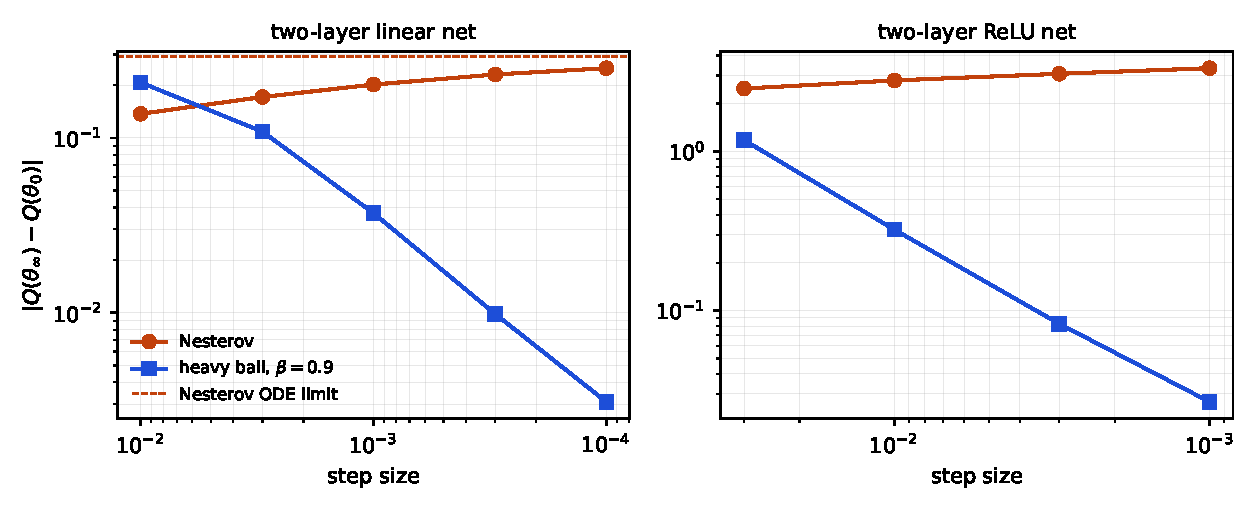
\includegraphics[width=\linewidth]{fig_dichotomy.pdf}
\caption{Drift of the conserved quantity against step size for Nesterov's method and for heavy ball with $\beta=0.9$, run to convergence. Left: $C_{00}$ for a two-layer linear network. Right: the balancedness of one neuron of a two-layer ReLU network.}
\label{fig:dichotomy}
\end{figure}

\section{Why the drift matters: implicit bias}\label{sec:bias}

For a two-layer diagonal linear network $w=u\odot v$, each $\Delta_i=u_i^2-v_i^2$ is conserved by gradient flow. Along the flow $\dot w_i=-\sqrt{\Delta_i^2+4w_i^2}\,\partial_iL$, which is mirror descent with $\phi''(w)=(\Delta^2+4w^2)^{-1/2}$. From $w_0=0$ on an underdetermined regression problem $Xw=y$ the limit is therefore
\[
w(\Delta)=\arg\min\Bigl\{\sum_i\phi_{\Delta_i}(w_i):Xw=y\Bigr\},
\]
which is the hyperbolic entropy picture of Woodworth et al.\ and Azulay et al.~\cite{woodworth2020,azulay2021}. Small $|\Delta|$ favours sparse solutions. The conserved quantities therefore are the implicit bias, and a bound on their drift is a bound on how far momentum can move it.

We trained a diagonal network with $n=20$, $d=60$, a 3-sparse target and $u_0=0.1$, $v_0=0$. \Cref{tab:bias} shows that the distance of the learned $w$ from the gradient flow solution $w(\Delta_0)$ grows with the drift of $\Delta$, and the $\ell_1$ norm grows with it. The heavy ball rows order by $\eta/(1-\beta)^2$, in agreement with \cref{thm:discbound} and with Papazov et al. When the drift is small, the gradient flow prediction from the final $\Delta$ is much closer to the learned solution than the prediction from the initial $\Delta$, by a factor of $26$ for plain gradient descent. When the drift is large neither prediction is accurate, because $\Delta$ changed along the path and the limit is not a Bregman projection for any single $\Delta$. Nesterov's drift is about $0.04$ at both step sizes, consistent with Observation~\ref{obs:dichotomy}.

\begin{table}[t]
\centering\small
\begin{tabular}{lrrrrrr}
\toprule
run & $\eta/(1-\beta)^2$ & $\max|\Delta_\infty-\Delta_0|$ & $\|w\|_1$ & $\|w-w^\ast\|$ & $\|w-w(\Delta_0)\|$ & $\|w-w(\Delta_\infty)\|$\\
\midrule
GD, $\eta=0.05$ & 0.05 & $1.1\times10^{-3}$ & 3.027 & 0.397 & $5.4\times10^{-3}$ & $2.0\times10^{-4}$\\
HB, $\beta=0.5$ & 0.2 & $5.7\times10^{-3}$ & 3.063 & 0.419 & $2.8\times10^{-2}$ & $1.4\times10^{-2}$\\
HB, $\beta=0.9$, $\eta=0.02$ & 2 & $2.8\times10^{-2}$ & 3.303 & 0.554 & 0.170 & 0.292\\
HB, $\beta=0.9$, $\eta=0.05$ & 5 & $6.5\times10^{-2}$ & 3.522 & 0.682 & 0.305 & 0.255\\
HB, $\beta=0.95$ & 12 & $9.8\times10^{-2}$ & 4.063 & 0.984 & 0.627 & 0.444\\
Nesterov, $s=0.05$ & & $4.5\times10^{-2}$ & 3.145 & 0.477 & 0.100 & 0.293\\
Nesterov, $s=0.01$ & & $4.2\times10^{-2}$ & 3.184 & 0.503 & 0.129 & 0.255\\
\bottomrule
\end{tabular}
\caption{Diagonal linear network, ground truth $\|w^\ast\|_1=2.4$. The gradient flow solution $w(\Delta_0)$ has $\ell_1$ norm $3.019$.}
\label{tab:bias}
\end{table}

\section{Numerical checks}\label{sec:numerics}

The scripts are in \texttt{numerics/}. The models are a two-layer ReLU network with four hidden units on 40 points in $\R^5$ and a two-layer linear network with widths $6\to4\to3$ on 30 points. ODEs are integrated with an eighth-order Runge--Kutta method at relative tolerance $10^{-11}$. The continuous identity \eqref{eq:hbid} holds to all printed digits for $m$ from $0.003$ to $1$. The discrete identity \eqref{eq:discid} holds to within $3\times10^{-13}$ on all four neurons of the ReLU network for four choices of $(\eta,\beta)$. The first bound of \cref{thm:discbound} holds in every case. The second bound needs $\eta\ell<2(1-\beta)$ for the smoothness constant $\ell$ measured along the run, and this fails for $\eta=0.005$, $\beta=0.97$, where $\eta\ell/(2(1-\beta))=2.1$. For that run the bound does not apply. The energy identity of \cref{thm:nest} holds to seven digits. The nuclear norm bound of Corollary~\ref{cor:matrix} holds with ratio about $0.65$ at three settings.

The third model is scale invariant, $L(w)=\frac1{2n}\sum_i(x_i^\top w/\|w\|-y_i)^2$ with $w\in\R^6$ and $n=30$, so $A=I$ and $Q=\|w\|^2$, with $\|w_0\|^2=4.63$. \Cref{tab:scaleinv} shows the dichotomy of Corollary~\ref{cor:dichotomy}. Heavy ball was run for $60/s$ steps and Nesterov for $4000/\sqrt s$ steps. The identity of \cref{thm:nag} holds to $2\times10^{-11}$ on this model and on the ReLU network.

\begin{table}[h]
\centering\small
\setlength\tabcolsep{4pt}\begin{tabular}{lrrrrr}
\toprule
step $s$ & $10^{-1}$ & $3\times10^{-2}$ & $10^{-2}$ & $3\times10^{-3}$ & $10^{-3}$\\
\midrule
Nesterov, $\|w_\infty\|^2-\|w_0\|^2$ & 8.19 & 9.74 & 10.78 & 11.54 & 11.97\\
heavy ball $\beta=0.9$, $\|w_\infty\|^2-\|w_0\|^2$ & 15.88 & 4.76 & 1.58 & 0.475 & 0.158\\
\bottomrule
\end{tabular}
\caption{Growth of the squared norm of scale-invariant weights. Heavy ball's growth is proportional to the step. Nesterov's grows towards a positive limit.}
\label{tab:scaleinv}
\end{table}

\section{Formalisation}\label{sec:lean}
{\sloppy

The directory \texttt{lean/} is a Lean~4 project on Mathlib. It builds with no \texttt{sorry}, and \texttt{\#print axioms} on the main theorems lists only \texttt{propext}, \texttt{Classical.choice} and \texttt{Quot.sound}. Parameters live in an arbitrary real inner product space and $A$ is a continuous linear map, so the results hold for every architecture at once.

\texttt{Discrete.lean} proves \cref{thm:disc} for an arbitrary schedule (\texttt{drift\_eq\_sum}, \texttt{P\_succ}), the identity \eqref{eq:discid} (\texttt{drift\_const}), both bounds of \cref{thm:discbound} (\texttt{drift\_bound\_const}, \texttt{sum\_sq\_le\_of\_descent}, \texttt{drift\_bound\_energy}), the discrete equality case (\texttt{drift\_scale\_invariant}) and \cref{thm:nestdisc} (\texttt{P\_nest}, \texttt{drift\_nesterov\_schedule}). \texttt{Continuous.lean} proves \eqref{eq:hbid}, its integrated form, the energy identity and \eqref{eq:hbbound} (\texttt{hb\_corrected\_deriv}, \texttt{hb\_identity}, \texttt{hb\_energy}, \texttt{hb\_drift\_bound}), and both identities of \cref{thm:nest} (\texttt{nesterov\_identity}, \texttt{nesterov\_energy}). These statements assume the trajectory and its velocity are differentiable with the stated derivatives and take the chain rule for $L$ as a hypothesis.

\texttt{LinearNet.lean} proves Corollary~\ref{cor:matrix} for matrices over arbitrary finite index types: the step identity for $C$ (\texttt{C\_step}), the recursion (\texttt{P\_succ}), the exact matrix identity (\texttt{drift\_matrix\_const}), its quadratic-form version (\texttt{quad\_drift}) and the bound $|\operatorname{tr}(X(C_N-C_0))|\le\frac{1+\beta}{1-\beta}\sum_j(\|V^{(1)}_j\|_F^2+\|V^{(2)}_j\|_F^2)$ for every $X$ with $|x^\top Xx|\le x^\top x$ (\texttt{trace\_drift\_bound}). The nuclear norm bound is the supremum of this over $X$, which is the standard duality between the trace and operator norms. That last step is not formalised. The file also checks that gradients of any loss of the form $\ell(W_2W_1)$ satisfy the orthogonality used (\texttt{orth\_of\_factor}).

\texttt{Nesterov.lean} proves \cref{thm:nag}: the polarisation identity (\texttt{Q\_extrap}), the recursion (\texttt{D\_succ}), the closed form with Nesterov's weights (\texttt{drift\_nag\_nesterov}), nonnegativity of the weights and the bound $w_i\ge i/4$ on the first half of the run (\texttt{wNest\_nonneg}, \texttt{wNest\_ge}), and the reduction to an initial block for $A\succeq0$ (\texttt{drift\_nag\_ge}). \texttt{NesterovLower.lean} proves \cref{thm:nestlower} as stated, including the position, velocity and error estimates of the early phase (\texttt{early\_bounds}, \texttt{err\_bound}, \texttt{kinetic\_lower}, \texttt{nesterov\_lower\_bound}). The final choice of $J$ in Corollary~\ref{cor:dichotomy} is elementary arithmetic and is not formalised.

Not formalised: the limits $T\to\infty$ in \eqref{eq:hblim} and \cref{thm:nest}, \cref{thm:first} and Lemma~\ref{lem:layer}, the duality step and the choice of $J$ mentioned above, and Observation~\ref{obs:dichotomy}, which is numerical.

}

\section{Limitations}

The bounds are uniform in time but loose for typical initialisations, by factors between about $3$ and $80$ in our runs, because $K$ has both signs. Proposition~\ref{prop:sharp} shows that no better constant exists in general. The constant in Corollary~\ref{cor:dichotomy} is smaller than the observed drift by seven orders of magnitude, and the dichotomy is proved only for positive semidefinite generators. For indefinite generators, including the rescaling symmetry of ReLU neurons, it rests on numerics. \Cref{thm:first} gives the first-order limit without a rate and needs the gradient flow to reach the global infimum. The discrete energy bound needs a smoothness constant along the trajectory, which neural network losses do not have globally. The implicit bias experiment uses one problem and one initialisation scale. Our search of prior work covered the papers cited here and searches on the main claims in October 2026. It was not exhaustive.

\begin{thebibliography}{99}
\bibitem{arora2019} S.~Arora, Z.~Li and K.~Lyu. Theoretical analysis of auto rate-tuning by batch normalization. ICLR 2019.
\bibitem{arora2018} S.~Arora, N.~Cohen and E.~Hazan. On the optimization of deep networks: implicit acceleration by overparameterization. ICML 2018.
\bibitem{azulay2021} S.~Azulay, E.~Moroshko, M.~S.~Nacson, B.~Woodworth, N.~Srebro, A.~Globerson and D.~Soudry. On the implicit bias of initialization shape: beyond infinitesimal mirror descent. ICML 2021.
\bibitem{du2018} S.~S.~Du, W.~Hu and J.~D.~Lee. Algorithmic regularization in learning deep homogeneous models: layers are automatically balanced. NeurIPS 2018.
\bibitem{josz2024} C.~Josz and X.~Li. Singular perturbation in heavy ball dynamics. arXiv:2407.15044, 2024.
\bibitem{kunin2021} D.~Kunin, J.~Sagastuy-Brena, S.~Ganguli, D.~L.~K.~Yamins and H.~Tanaka. Neural mechanics: symmetry and broken conservation laws in deep learning dynamics. ICLR 2021.
\bibitem{lyu2025} B.~Lyu, H.~Wang, Z.~Wang and Z.~Zhu. Effects of momentum in implicit bias of gradient flow for diagonal linear networks. AAAI 2025.
\bibitem{marcotte2023} S.~Marcotte, R.~Gribonval and G.~Peyr\'e. Abide by the law and follow the flow: conservation laws for gradient flows. NeurIPS 2023.
\bibitem{marcotte2024} S.~Marcotte, R.~Gribonval and G.~Peyr\'e. Keep the momentum: conservation laws beyond Euclidean gradient flows. ICML 2024.
\bibitem{medeiros2026} D.~N.~Medeiros. Conservation law breaking at the edge of stability: a spectral theory of non-convex neural network optimization. arXiv:2604.07405, 2026.
\bibitem{papazov2024} H.~Papazov, S.~Pesme and N.~Flammarion. Leveraging continuous time to understand momentum when training diagonal linear networks. AISTATS 2024.
\bibitem{polyak1964} B.~T.~Polyak. Some methods of speeding up the convergence of iteration methods. USSR Computational Mathematics and Mathematical Physics 4(5), 1964.
\bibitem{shi2022} B.~Shi, S.~S.~Du, M.~I.~Jordan and W.~J.~Su. Understanding the acceleration phenomenon via high-resolution differential equations. Mathematical Programming 195, 2022.
\bibitem{su2016} W.~Su, S.~Boyd and E.~J.~Cand\`es. A differential equation for modeling Nesterov's accelerated gradient method. Journal of Machine Learning Research 17, 2016.
\bibitem{tanaka2021} H.~Tanaka and D.~Kunin. Noether's learning dynamics: role of symmetry breaking in neural networks. NeurIPS 2021.
\bibitem{wan2021} R.~Wan, Z.~Zhu, X.~Zhang and J.~Sun. Spherical motion dynamics: learning dynamics of normalized neural network using SGD and weight decay. NeurIPS 2021.
\bibitem{woodworth2020} B.~Woodworth, S.~Gunasekar, J.~D.~Lee, E.~Moroshko, P.~Savarese, I.~Golan, D.~Soudry and N.~Srebro. Kernel and rich regimes in overparametrized models. COLT 2020.
\end{thebibliography}

\end{document}
